\chapter{Сложные структуры данных}
\label{ch:advanced-ds}

\section{Префиксные деревья}
\label{sec:trie}
Префиксное дерево (trie) — структура данных, позволяющая хранить ассоциативный массив, ключами которого являются, как правило, строки. В отличие от двоичных деревьев поиска не обязательно хранить ключ в узлах дерева, так как в префиксном дереве по позиции узла можно вычислить ключ, ассоциированный с ним. Все потомки узла имеют общий префикс, представленный этим самым узлом.

Ниже на рисунке представлено префиксное дерево с некоторыми английскими словами в качестве ключей.
\begin{center}
  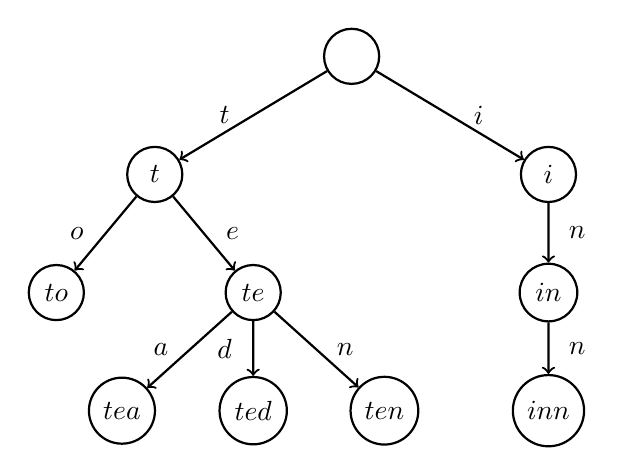
\begin{tikzpicture}[minimum size=7mm,
                      circle,thick,
                      edge from parent/.style={->,draw,thick},
                      level/.style={sibling distance=50mm/#1}]
    \node [draw] {}
      child { node [draw] {$t$}
        child { node [draw] {$to$}
          edge from parent
            node[left] {$o$}
        }
        child { node [draw] {$te$}
          child { node [draw] {$tea$}
            edge from parent
              node[left] {$a$}
          }
          child { node [draw] {$ted$}
            edge from parent
              node[left] {$d$}
          }
          child { node [draw] {$ten$}
            edge from parent
              node[right] {$n$}
          }
          edge from parent
            node[right] {$e$}
        }
        edge from parent
          node[left] {$t$}
      }
      child { node [draw] {$i$}
        child { node [draw] {$in$}
          child { node [draw] {$inn$}
            edge from parent
              node[right] {$n$}
          }
          edge from parent
            node[right] {$n$}
        }
        edge from parent
          node[right] {$i$}
      };
  \end{tikzpicture}
\end{center}

В качестве ключей могут использоваться не только строки, но и любая последовательность. Время вставки, удаления и поиска в префиксном дереве равно $O(m)$, где $m$ — длина ключа.

\lstinputlisting[style=ocamlstyle,caption=Реализация префиксного дерева]{src/advanced-ds/trie.ml}

\begin{ocamllst}{Пример использования}{}
# let root = make_root ()
# let root = insert root "tea" "tea"
# let root = insert root "ted" "ted"
# let root = insert root "ten" "ten"
# let root = insert root "inn" "inn"
# let root = insert root "te" "te"
# let root = insert root "" "" ;;

value root : trie string =
  {value=Some "";
   children=
    [('t',
     {value=None;
      children=
       [('e',
        {value=Some "te";
         children=
          [('n', {value=Some "ten"; children=[]});
           ('d', {value=Some "ted"; children=[]});
           ('a', {value=Some "tea"; children=[]})]})]});
     ('i',
     {value=None;
      children=
       [('n',
        {value=None; children=[('n', {value=Some "inn"; children=[]})]})]})]}

# let root = remove root ""
# let root = remove root "te"
# let root = remove root "inn"
# let root = remove root "ten"
# let root = remove root "ted"
# let root = remove root "tea" ;;

value root : trie string = {value=None; children=[]}
\end{ocamllst}
